\chapter{Geometric Series}

In this chapter we will discuss one of the simplest and most useful
types of infinite series, the geometric series.  They are derived
from instances where \textbf{geometric growth} occurs, this is growth that
is proportional to the current value, i.e the growth rate is constant. (Here
we are looking at the discrete situation, in a continuous situation a
differential equation for constant growth rate produces exponential
functions as solutions.)

A simple example of geometric growth is
interest accrued annually on a bank account.  Each year we take the
amount of money in the account the value of the account and multiply
it by the interest rate and add it to the value to get a new value.
Therefore the constant of proportionality is one plus the interest
rate.
\begin{Example}
If you put {\$}$100$ into a savings account that earned $3$\% interest
accrued annually, how much would you have after one year? two years?
$n$ years?

\solution
Let $p_{n}$ be the value of our account at time n, so $p_{0}=100$
since we begin initially with {\$}$100$.  Next at the end of one year we
earn 3\% interest on this account so $p_{1}=(1.03)\cdot p_{0}=(1.03)
\cdot 100$, hence $p_{1}$ is proportional to $p_{0}$ with the
constant of proportionality being 1.03. This process repeats so that
$p_{2}=(1.03) \cdot p_{1}=(1.03)^{2} \cdot 100$.  At this point we
notice a pattern $p_{n}=(1.03)^{n} \cdot 100$.
\end{Example}

As a second example of geometric growth we consider university
scholarships which come from endowments.  In this case, an endowment (a
fixed sum)
is given to the university. A scholarship then is funded from the interest
of this money (without using up the money, the scholarship therefore exists
forever).

\begin{Example}[Endowments]
Delighted by the calculus course he took at CSU, an alumnus wants to endow a
scholarship for mathematics students that will pay {\$}$2000$ each year. The
university guarantees an interest rate of $5$\% per year.
How much must the alumnus donate to guarantee this
scholarship will be available forever?

\solution
If we let $x$=the value of the endowment, then after one year the
endowment is worth $1.05 \cdot x$ and we want to give a {\$}$2000$
scholarship, so we want $1.05x=x+2000$.  Therefore the endowment
will never be touched and the scholarship is funded by the interest
earned.  Solving this equation we get $0.05x=2000$ which gives us
that $x=40,000$.  Therefore the alumni must give an endowment of
{\$}$40,000$ to guarantee the scholarship is funded forever.
\end{Example}
\medskip

A geometric series now is a series whose terms show geometric growth, i.e.
$s_n=r\cdot s_{n-1}$ for a constant $r$ independent of $n$.
This type of series has applications in several fields
including physics, biology, economics and finance. We will look at a
few examples of where geometric series occur in our everyday lives
including: repeating decimals and calculating dosage of medicine.
\begin{Definition}
Let $r$ be a ratio and $a$ any nonzero constant. A \defini{geometric series}
is a series of the form
\[
a+ ar + ar^{2}+ \ldots + ar^{n-1}+ \ldots = \sum_{n=1}^{\infty}
ar^{n-1} =a\sum_{n=1}^\infty r^{n-1}=a\sum_{n=0}^\infty r^n
\]
\end{Definition}

As an example of a geometric series we look at the ``Race course paradox'' of
Zeno\mynote{Zeno of Elea, Greek philosopher, ca. 490 BC - ca. 430 BC}.
Suppose a runner wanted to travel a given distance, say one kilometer. Then
he must first travel the first half kilometer, and the next half kilometer
remains.  Next the runner must travel half of the next half kilometer -- a
quarter kilometer  -- and the next quarter kilometer remains. It might seem
(so claimed Zeno) as if the runner never reaches the goal.

\begin{figure}[h]
\begin{center}
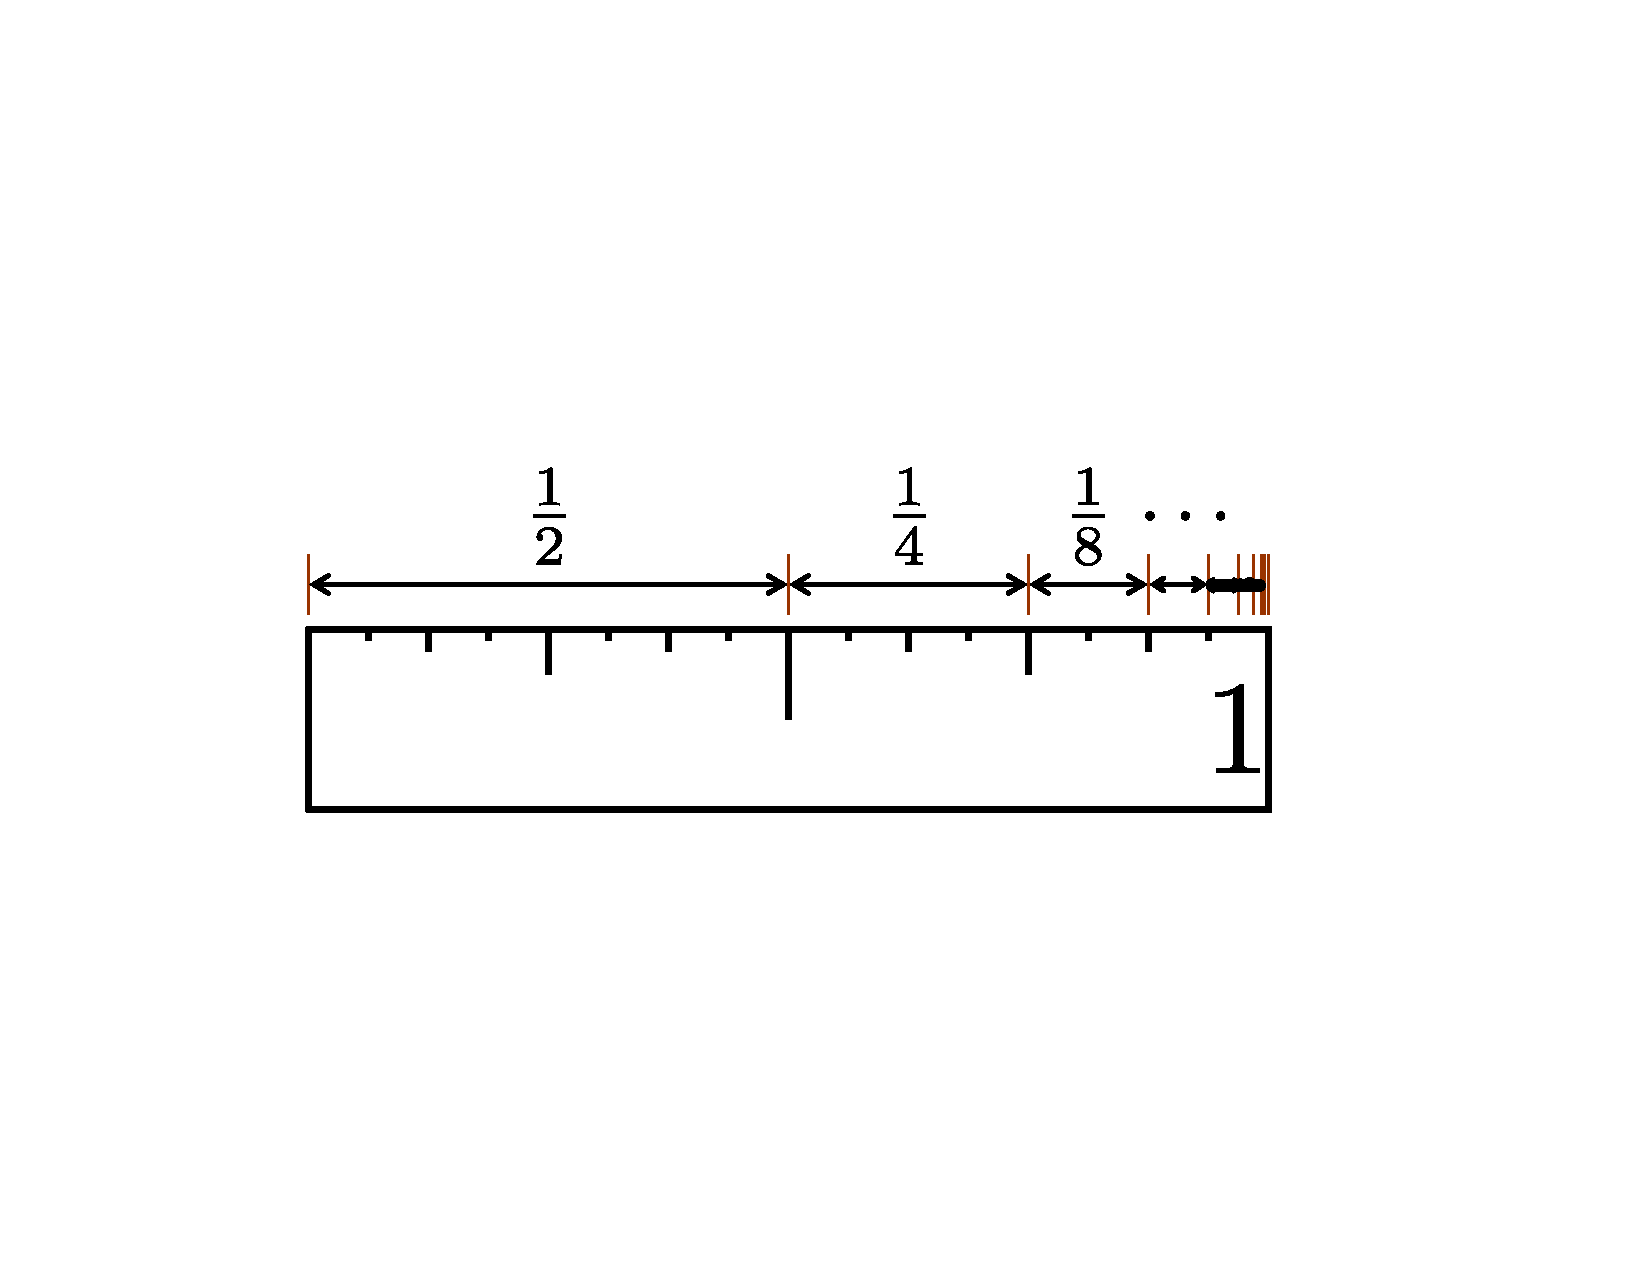
\includegraphics[width=5cm]{GeometricSegment.pdf}
\end{center}
\end{figure}

However if we look at the distance traveled after $k$ iterations, we
get a geometric sum with ratio $\frac{1}{2}$:
\[
\frac{1}{2}+\frac{1}{4}
+\frac{1}{8}+\frac{1}{16}+\cdots+\frac{1}{2^k}
\]
If the process continues infinitely many times, we thus get get the
following formula for the distance traveled:
\[
\frac{1}{2} + \frac{1}{4} + \frac{1}{8} + \ldots + \frac{1}{2^{n}} +
\ldots = \sum_{n=1}^{\infty} \frac{1}{2^{n}}
\]
We will see that this sums up to $1$ (i.e. the full distance is traveled,
resolving the paradox).

Notice that there is a slight shift in this formula from the one
given in the definition of a geometric series in that we start not
with $r^0=1$ but with $r^{1}=\frac{1}{2}$ while in the definition
this power is zero.  This can be fixed by letting the constant a be
$\frac{1}{2}$, This sort of index change arises often enough that we
will first look at how we can manipulate such infinite sums.

\section*{Reindexing a Series}
We begin this discussion with a brief reminder about the $\Sigma$ notation
for sums.
Given $\displaystyle{\sum_{n=1}^{k} a_{n}}$ we call n the
\textbf{index of summation}, $a_{n}$ the \textbf{$n^{th}$ term} of
the sum, and the \textbf{upper and lower bounds of summation} are k
and 1
respectively.  \\

Now we consider reindexing our infinite series, notice in the
following examples we are working with geometric series, however
this algorithm will be useful with other
types of series that will be discussed later. \\

Most of the infinite series we have seen so far have a lower bound
of summation of one, however their are times when we are given an
infinite series where the lower bound of summation will be a value
other than one. We consider first a geometric series which does not
have a lower bound of one: $$ \frac{-1}{27} + \frac{1}{81} -
\frac{1}{243} + \ldots + (\frac{-1}{3})^{n-1} + \ldots =
\sum_{n=4}^{\infty} (\frac{-1}{3})^{n-1} $$ This is still a
geometric series, however our definition requires the series to have
the form $\displaystyle{\sum_{n=1}^{\infty} ar^{n-1}}$, so
reindexing is required. To reindex a series we follow the following
basic algorithm:
\begin{Algorithm}[Reindexing a series]\ 
\begin{itemize}
\item[1] Choose a new letter to be the index of summation (m)
\item[2] Relate m to the original index of summation (n) such that when
n=4 we have m=1.  So we have the equation m=n-3.
\item[3] Solve for original index of summation (n) and substitute into
the $n^{th}$ term of the sum: $$ n=m+3 \Rightarrow
\sum_{m=1}^{\infty} (\frac{-1}{3})^{m+3-1} = \sum_{m=1}^{\infty}
(\frac{-1}{3})^{m+2} $$ Notice if the upper bound of summation were
finite we would have to decrease its value by 3 as well, however
since we are summing to infinity our upper bound of summation will
remain infinite.
\item[4] Solve for an a such that the power on r is m-1. $$
\sum_{m=1}^{\infty} (\frac{-1}{3})^{m+2} = \sum_{m=1}^{\infty}
(\frac{-1}{3})^{3} \cdot (\frac{-1}{3})^{m-1}$$ since m-1+3=m+2.
\end{itemize}
\end{Algorithm}
Therefore $a=(\frac{-1}{3})^3 = \frac{-1}{27}$ and $r=\frac{-1}{3}$
so we have a geometric series of the form
$\displaystyle{\sum_{m=1}^{\infty} ar^{m-1}}$.  Notice that in this
example the ratio was negative, therefore a geometric series can
have negative or positive r values. We now look at another example
of this reindexing algorithm before we develop an equation for the
value of a geometric series.

\begin{Example}
Consider the series $\displaystyle{\sum_{n=9}^{\infty}
\frac{4}{2n+3}} $, rewrite
this series so that the lower bound of summation is n=1.

\solution
Let $m=n-8$, then $n=m+8$ so we have
$\displaystyle{\sum_{m=1}^{\infty} \frac{4}{2(m+8)+3} =
\sum_{n=1}^{\infty} \frac{4}{2m+19}}$
\end{Example}

Using this algorithm we can always manipulate a given geometric
series so that it can be written in the form
$\displaystyle{\sum_{n=1}^{\infty} ar^{n-1}}$ or equivalently
$\displaystyle{\sum_{n=0}^{\infty} ar^n}$ next we consider how to
calculate the value of this series.

\section*{The Formula for the Geometric Series}
In this section we will derive a general formula for the value of
$\displaystyle{ \sum_{n=0}^{k} ar^{n}}$. We can apply this in the
limit case $k=\infty$ to get the value of an infinite series, for
example to show that the series $\displaystyle{\sum_{n=1}^{\infty}
\frac{1}{2^n}}$ from Zeno's paradox has value $1$.

\begin{Definition}
The \textbf{ $k^{th}$ partial sum $s_{k}$} of a Geometric series
$\displaystyle{\sum_{n=0}^{\infty} ar^{n}}$ is the (finite) sum of
the first $k$ terms:
\[
s_{k} = a + ar + ar^{2} + \ldots + ar^{k-1} =
\sum_{n=0}^{k-1} ar^{n}
\]
\end{Definition}
Using this definition we can consider the {\em sequence} $s_{1},
s_{2}, s_{3}, \ldots , s_{k}, \ldots $ of partial sums,  which
converges to $\displaystyle{\sum_{n=0}^{\infty} ar^{n}}$, since
$\displaystyle{\lim_{k \rightarrow \infty} s_{k} = \lim_{k
\rightarrow \infty} \sum_{n=0}^{k-1} ar^{n} = \sum_{n=0}^{\infty}
ar^{n}}$. Therefore, once we know a formula for the value of $s_{k}$
we can compute the value of $\displaystyle{\sum_{n=0}^{\infty}
ar^{n}}$ as the limit.

We begin by considering
\[
s_{k}=a + ar + ar^{2} + \ldots + ar^{k-1}
\]
and
\[
rs_{k} = ar + ar^{2} + ar^{3} + \ldots + ar^{k}.
\]
Notice that $s_{k}$ and $rs_{k}$ share several terms in common, in
fact
\[
s_{k}-rs_{k}= (a + ar + ar^{2} + \ldots + ar^{k-1}) - (ar +
ar^{2} + ar^{3} + \ldots + ar^{k}) = a -ar^{k}
\]
Now if we factor both sides of this equation, we get
\[
s_{k}(1-r)=a(1-r^{k}).
\]
As
long as $r \neq 1$ we can divide both sides by $(1-r)$ to get
\begin{center}
\fbox{\begin{minipage}{3in}
\Large
\[
s_{k}=\sum_{n=0}^{k-1}ar^n=a\frac{1-r^{k}}{1-r}.
\]
\end{minipage}}
\end{center}

(What happens in the case where r=1?
We get $s_{k}= a + a(1) + a(1)^{2} + \ldots + a(1)^{k-1}=ka$.)
\medskip

Before we go on to get a formula for the infinite sum, we see
how the formula for $s_{k}$ might be used on its own:
\begin{Example}[The magnitude of repeated growth]
Suppose we are given a chessboard and place one grain of rice on
the first square, two grains of rice on the second square, four
grains of rice on the third square continuing on so that there are
$2^{n-1}$ grains of rice on the $n^{th}$ square.  How many grains of
rice are on the chess board? (There are $8\cdot 8=64$ squares on a chess
board.) 
%\begin{figure}
% \epsfig{file=Chess-board-walnut.jpg,scale=.8}
%\end{figure}

\solution
Since there are 64 squares on the chess board, we want to compute
$s_{64}$.  Our ratio is 2 and $a$ is one, hence we are asked to find
\[
s_{64}=1+2+4+ \ldots +2^{63} =
\frac{1(1-2^{64})}{1-2} = 1.84467 x 10^{19}
\]
\end{Example}

A similar calculation underlies the repayment of loans or mortgages:

\begin{Example}[Paying back a loan]
Suppose we take out a loan of $L$ dollars which is paid back
periodically (typically monthly). The periodic payment is $a$
dollars, the fixed interest rate \textit{per period} is $i$. If
$b_k$ is the loan sum outstanding after $k$ time periods, we have
that
\[
b_{k+1}=b_k\cdot (1+i)-a.
\]
Using $b_0=L$ and setting $r=1+i$, in the first step we have
\[b_{1}=Lr-a\] we then continue on to the next step where we
get
\begin{eqnarray*}
b_{2}&=&b_{1}(r)-a 
=(Lr-a)(r)-a \\
&=&Lr^{2}-(a+ar)
\end{eqnarray*}
We might be starting to notice a pattern, however it becomes obvious
in the next step
\begin{eqnarray*}
b_{3}&=&b_{2}(r)-a 
=(Lr^{2}-(a+ar))(r)-a \\
&=&Lr^{3}-(a+ar+ar^{2})
\end{eqnarray*}
At this point we can solve this recursion to
\[
b_k=L\cdot r^k-\left(a+ar+ar^2+\cdots+ar^{k-1}\right)
=L\cdot r^k-\sum_{n=0}^{k-1}ar^n
\mathop{=}\limits^{\mbox{\quad Sum formula\quad}}L\cdot r^k-a\frac{1-r^k}{1-r}.
\]
A bank now would set $b_m=0$ (where $m$ is the time after which the loan
should be paid off, e.g. $m=12\cdot 30=360$ for a 30 year mortgage)
and solve for $a$ to determine the
necessary monthly repayment, given the loan sum and interest rate.

For example, if we have a mortgage of $L=\$200,000$, an annual
interest rate of $6$\% (leading to a monthly rate of
$i=.06/12=0.005$, i.e. $r=1.005$) and a monthly repayment
sum\mynote{Moralistic remark: Incidentally, initial interest amounts
to {\$}$1000$ per month at the start of the loan. An
\textit{interest only} loan thus does not save much and is a very
bad deal!} of $a=\$1,200$, we find that the outstanding sum after
$k$ months is
\[
b_k=200,000\cdot{1.005^k}-1,200\frac{1.005^k-1}{0.005}
=200,000\cdot{1.005^k}-240,000\left(1.005^k-1\right).
\]
After $10$ years ($120$ months) this leaves an outstanding amount of
{\$}$167,224.13$, after $20$ years {\$}$107,591.82$, roughly
half\mynote{In general, this means that a loan is paid off half
after roughly $\frac{2}{3}$ of its planned life time}, after $30$
years {\$}$-903.00$ (i.e. the loan is paid off after $30$ years less
one month\mynote{The total cost of the loan then will have been
{\$}$430,800$, more than double the loan amount. (Though inflation
means that the actual value will be less.)}).

If the interest rate instead was $7$\% annually ($i=.07/12=0.005833$
monthly), we get with same repayment sum a remaining loan amount of
{\$}$159,256.18$ after $30$ years, which is not even halfway paid
off. A monthly repayment sum of {\$}$1330$ would be
needed\mynote{I.e. a change of one percentage point in the
interest rate increased the monthly payment (and thus the total loan
cost) by $10$\%! No wonder people go bonkers about interest rates.}
to have the loan paid off after $30$ years.
\end{Example}

Now since we saw earlier that the sequence $s_{1}, s_{2}, s_{3},
\ldots, s_{k}, \ldots$ of partial sums converges to
$\displaystyle{\sum_{n=1}^{\infty} ar^{n-1}}$, we can use the
formula just derived to compute a value for the limit of a geometric series.

\begin{center}
\fbox{\begin{minipage}{\textwidth}
\begin{Theorem}
The geometric series $\displaystyle a + ar + ar^{2}+ \ldots +
ar^{n-1} + \ldots =\sum_{n=1}^{\infty} ar^{n-1}$ converges to
$\displaystyle\frac{a}{1-r}$ when $|r|<1$, and diverges otherwise.
\end{Theorem}
\end{minipage}}
\end{center}
\begin{proof}
\textbf{Case 1:} If $|r|<1$ then $|r|^{k} <1$, and as $k$ gets
larger this will cause $|r^{k}|$ to get smaller and yield
$\displaystyle\lim_{k \rightarrow \infty} r^{k}=0$. Thus, by the rules for
limits,
\[
\lim_{k\to\infty} s_k=
\lim_{k \rightarrow \infty} \frac{a (1-r^{k})}{1-r} =
\frac{a(1-0)}{1-r}=\frac{a}{1-r}.
\]
\\
\textbf{Case 2:} When $|r| \geq 1$ then $|r|^{k} \geq
1$. Therefore when $k$ tends to infinity the numerator $a(1-r^{k})$
tends to plus or minus infinity, and the denominator $1-r$ is a fixed
value. So $\displaystyle{\lim_{k \rightarrow \infty}
\frac{a
(1-r^{k})}{1-r}}$ diverges.
\end{proof}

Now that we have a formula for the value of a geometric series let
us verify the solution to the Zeno's paradox example.  We are
looking at $\displaystyle{\sum_{n=1}^{\infty}\frac{1}{2^n}}$. First
notice that this sum is not in the correct form,  we must factor
$(\frac{1}{2})$ out of the $n^{th}$ term.  We get
$\displaystyle{\sum_{n=1}^{\infty} ( \frac{1}{2})^{n} =
\sum_{n=1}^{\infty}(\frac{1}{2})\cdot(\frac{1}{2})^{n-1}
=\sum_{n=0}^{\infty} (\frac{1}{2}) \cdot (\frac{1}{2})^{n}}$, hence
$a=\frac{1}{2}$ and $r=\frac{1}{2} < 1$ so this series converges to
\[
\frac{a}{1-r} =
\frac{\frac{1}{2}}{1-\frac{1}{2}}=\frac{\frac{1}{2}}{\frac{1}{2}}=1.
\]

Next we will look at some interesting examples where we can use this
formula.

\section*{Examples}
In this section we will look at how people may use geometric series
in real life applications.

In our first example we
look at how much
medication will remain in a persons body after taking medication at
regular intervals
\begin{Example}[Repeated Drug Dosage]
A CSU student comes down with bacterial laryngitis, the student goes
to the Healthcenter to see a doctor who prescribes 250mg doses of
antibiotics that the student must take every six hours over the next
several days.  Since the body will digest the antibiotics between
doses and it is known that 5 percent of the drug remains in the body
at the end of six hours, how can we calculate the quantity of the
drug that remains in the student after the fifth dose? At the end of
five full days on the drug?

\solution
Let us begin by looking at the quantity of the drug in the body
after each dose.  Let $q_{n}$ represent the quantity of the drug in
the students body after the $n^{th}$ dose.  Initially $$ q_{1}=250$$
at the next dose we will have 5\% of that 250mg remaining and
another 250mg is taken, so $$q_{2}=250(0.05)+250$$ At the third dose
we have 5\% of $q_{2}$ remaining and another 250mg is taken, so
therefore
\begin{eqnarray*}
q_{3}&=&0.05 \cdot q_{2} +250 =0.05(250(0.05)+250) +250\\
&=&250(0.05)^{2} + 250(0.05) + 250.
\end{eqnarray*}
Now on the fourth dose
$q_{4}$ we have $0.05 \cdot q_{3}$ remaining in the body and another
250mg is taken.
\begin{eqnarray*}
q_{4}&=&0.05 \cdot q_{3} + 250
=0.05(250(0.05)^{2} + 250(0.05) + 250) + 250\\
&=&250(0.05)^{3} + 250(0.05)^{2} + 250(0.05) + 250.
\end{eqnarray*}
Notice at this point that a
pattern has developed, we have $$q_{n}=s_{n}=\sum_{k=1}^{n}
250(0.05)^{n-1}$$ Therefore we can use our formula
$s_{n}=\frac{a(1-r^{n})}{1-r}$ to calculate
$q_{n}=\frac{250(1-0.05^{n})}{1-0.05}$.  With this information we
can calculate $q_{5}=\frac{250(1-0.05^{5})}{1-0.05} = 263.1578125$mg
in the students body after 5 doses.  If the student continues to
take the antibiotic for 5 full days or 20 doses they will have
$q_{20}=\frac{250(1-0.05^{20})}{1-0.05}=263.1578947$mg. \\

Suppose the student continued to take this drug forever, how much
medication would there be in the students body at each dose?\\

This question is asking us to compute
$\displaystyle{\sum_{n=1}^{\infty} 250(0.05)^{n-1}}$ which luckily
for the student $0.05<1$ will converge to a finite number of
$\frac{250}{1-0.05}=263.1578947$mg. Since $0.05^{20}=9.536743 x
10^{-27}$ which is practically zero, we get the same value up to the
ten-millionth place if the student took the medication forever as we
got when the student took the medication for five days.

\end{Example}

\begin{Example}[Repeating Decimal]
Express the repeating decimal $0.\overline{08}$ as a fraction of two integers.

\solution
To express $0.\overline{08}$ as a fraction we first notice that $08$
is the repeated value, so we want to break up $0.\overline{08}$ into
a sum of the repeated values.  Therefore we have $0.\overline{08}=
0.\underline{08}+ 0.00\underline{08}+ 0.0000\underline{08}+ \ldots$.
Once we have this written as a sum we can now write each term in the
sum as a fraction, hence we have $0.\underline{08}=\frac{8}{100}$,
$0.00\underline{08}=\frac{8}{10,000}=\frac{8}{100^{2}}$, and
$0.0000\underline{08}=\frac{8}{100^{3}}$.  Using this information we
should recognize a pattern $$0.\overline{08} = \frac{8}{100} +
\frac{8}{100^{2}} + \frac{8}{100^{3}} + \ldots = \sum_{n=1}^{\infty}
\frac{8}{100^{n}}$$ However at this point we notice that we have a
geometric series which is not written in the correct form for us to
apply our formula.  If we factor out $(\frac{8}{100})$ we get
$\displaystyle{\sum_{n=1}^{\infty}
(\frac{8}{100})(\frac{1}{100})^{n-1}}$ which is now in the correct
form. This gives $r=\frac{1}{100} <1$ so our geometric series
converges and since $a=\frac{8}{100}$ the series converges to
$$\frac{\frac{8}{100}}{1-\frac{1}{100}}=\frac{\frac{8}{100}}{\frac{99}{100}}=\frac{8}{99}=0.\overline{08}$$
Being able to express a repeating decimal as a fraction is useful
when we are calculating with a large number of values where the
precision of the answer is vital since a fraction will not have
any round off error.  \\
\end{Example}

Another paradox due to Zeno initially seems even more puzzling, which is the
reason we consider it last.
Achilles, the fastest runner in ancient Greece, runs 100 times as
fast as the Tortoise. But --- so the paradox claims --- if the
Tortoise is given an advance, Achilles will never be able to pass
the Tortoise.

\begin{Example}[Achilles and the Tortoise]
Suppose that Achilles runs
$10 m/s$ and the Tortoise only $0.1 m/s$, furthermore the Tortoise is given
a head start of $100m$.
After $10$ seconds, Achilles has reached the place where the Tortoise
started. But in this time, the Tortoise has run $1m$ ahead. Achilles will
reach this distance in $0.1$ seconds. But then the Tortoise has moved
another $0.01m$. Achilles will take $0.001$ seconds to reach this, and so
on. He will never reach the Tortoise. Where is the error in this argument?

\solution
The paradox is resolved, if we realize what time period is considered:
All events take place within
\[
10+0.1+0.001+\cdots=10\sum_{n=0}^\infty
\frac{1}{100^n}=\frac{10}{1-\frac{1}{100}}=\frac{1000}{99}=10.\overline{10}
\]
seconds. This is exactly the time {\em when Achilles reaches (and
overtakes!) the Tortoise}. The paradox arises from the implicit
(and wrong, as we have calculated!)
suggestion, that it describes the events for all time.
\end{Example}

\section*{EXERCISES}

\begin{multicols}{2}
\paragraph{1.}
What monthly payment is needed to pay a car loan of \$ $15,000$ off after 48
months if the interest rate is $7$\%?

\paragraph{2.}
A standard method for valuing a business (excluding any inventory) is the
``discounted cash flow'' method: The value of the business itself is the
present day value of its future earnings, discounted by an assumed interest
rate, i.e. the amount of money that would have to be invested at an assumed
interest rate to get the same income as the business.

Calculate the present day value of a business whose annual earnings are
{\$}$50,000$, assuming an interest rate of $5$\%.

\paragraph{3.}
The goverment -- due to an election year in spending mode --
enacts a stimulus package that puts \$150 billion back into
the economy.
We assume that all the people who have extra
money to spend would spend 80\% of it and save
20\%. Thus, of the extra income generated by the package,
\$$150\cdot\frac{4}{5}$ billion = \$120 billion would be spent again and
so become extra income to someone else. Assume that
these people also spend 80\% of their additional income
(which would be \$$96=120\cdot\frac{4}{5}=150(\frac{4}{5})^2$ billion) and so on.

\noindent 
a) Let $C=150$ be the amount of the stimulus package (in billion dollars)
and $r=4/5$ the spending factor. Write down an infinite sum, involving $C$
and $r$, for the amount of money added to the economy.

\noindent
b) Calculate the value for the infinite sum in a).
\end{multicols}

